The planned listening tests were performed on a total of twelve participants, out of which ten were usable, with ages ranging from 21 to 30. In most of the tests, the overall user experience was deemed intuitive. There was some degree of confusion with regard to the features of the UI the participants were presented with, in particular the cubes used to mark which way the participant was facing. More than half of the subjects tested at least initially expected the sounds to come from these markers, and some mentioned that sounds continued to appear to originate from them even after they had been made aware of their purpose as just markers. In future tests, UI elements or position indicators should not have such a physical presence. A shortened version of the test was performed to allow the participants to acclimatise to the space, as well as to allow them to clarify any points of uncertainty before beginning the test proper. The tests themselves then took in between thirteen and nineteen minutes, and the primary bottleneck was the time spent preparing the next sample and fetching the modified HRTF data which was dependent on network speeds at the time. Ideally, any future versions of the test would be more self-contained. If the entirety of the process could be user-controlled, as opposed to requiring regular interaction between the subject and myself, then it may help the user to be better immersed in the process - perhaps producing better results. 

As mentioned in previous chapters, the primary metric for whether or not this implementation can be deemed effective is based upon the degree to which the severity of a participant's localisation errors decrease over time, if they decrease at all. This chapter will begin by investigating whether or not this is the case by reviewing the data captured during the listening tests. After this, an additional section will investigate the aforementioned relationship between PCW adjustment and localisation, to this end I have compared PCW values and perceived/actual source positions before and after different adjustment in an attempt to ascertain whether or not this is something worth additional study.

\section{Localisation Error Over Time}
In order to properly analyse this metric I am looking at the average total error value for each of the eight source positions. This error value is the angular error that comes from subtracting the perceived source position from the actual source position. These two values are then made positive if either one is negative, so as to better represent the total error in degrees, and summed to produce a combined error value. This process is performed for every participant, and the mean error value for each measurement over the course of the test from each direction is then calculated based on that data. These mean error rates over time can then be plotted as in figure 4.1. 

\begin{figure}
	\caption{The average error rate over each direction.}
	\centering{
		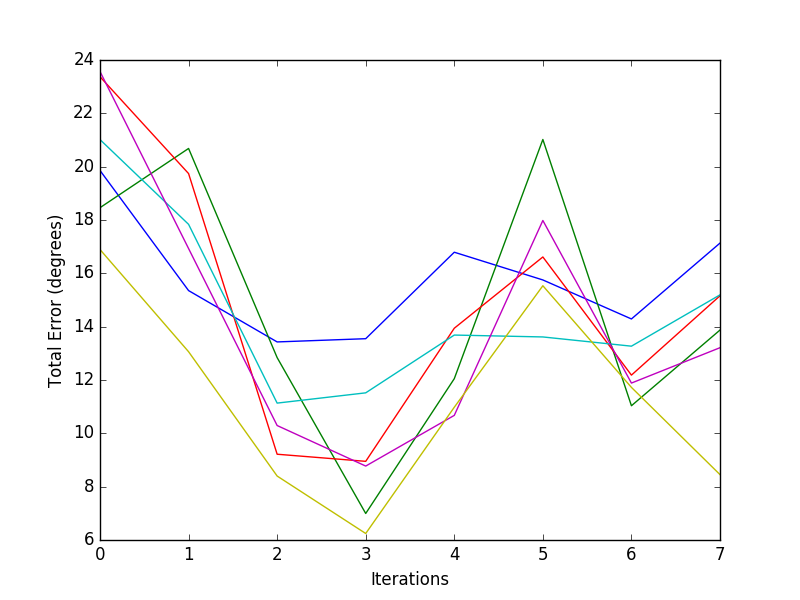
\includegraphics[scale=0.6]{average_error_each_direction}
	}
\end{figure}

On this chart each line represents a source position, and tracks how, on average, localisation errors for samples played from that source position changed over the course of the listening test. When displayed like this we can see something of a reduction in the overall errors for most source positions, but the short test length makes it unclear how close to zero these values would get or how long it would take. What we can see at play is the self-correcting quality afforded to the algorithm through knowledge of the history of previous changes. For almost all of the directions there are large spikes where the algorithm explores a sub-optimal child state and the participant's subsequent localisation attempt fares more poorly, in all cases but one (the black line representing the [-45.0, 135.0] source position) this mistake is quickly rectified as the algorithm makes adjustments in the opposite direction. Based on this and the slight overall trend down, it would not be unreasonable to expect that on a long enough timeline, the error rate would eventually get close to zero. If successive child states could be selected more intelligently, then it's quite possible that these kinds of mis-steps could be minimized further, reaching a more effectively individualised HRTF sooner.

It's also worth noting that three of the four directions with the most promising results were situated in front of the participant: [-45.0, 45.0], [45.0, 45.0], and [-45.0, -45.0]. This might stem from the much-documented front-back confusion common in non-individualised HRTFs, leading to poor average error rates for sources positioned behind the participant. Future implementations that are better able to account for head movement, allowing the participant small movements to aid in their localisation attempts, might produce better results, here. There is an exception to this in position [45.0, 135.0], which may have something to do with the starting HRTF used. Further research would be necessary to identify whether this is truly the case, but it would be interesting to investigate whether or not it is possible to generate a better base HRTF to begin this process with.

\section{Relationships Between PCs and Localisation Errors}
The ideal outcome when investigating this relationship would be to find a very clear indication of some correlation between certain combinations of adjustments to subsets of the available PCWs, and a change in apparent sound source. The starting dataset for this analysis drew from all the data captured, which was then sorted into a matrix in the shape [(Subjects x Directions) x Test iterations]. The data of interest from these tests was how the subject's perception of the location of the sound changed - in which direction and by how much - and which PCWs were adjusted to elicit that change. 

To this end, the six tests for each direction for each subject were organised into five pair objects, each of which contained the PCWs and the perceived location of the sound before and after. Because the location information in each pair object represented an apparent source position, fixed to the inside of a sphere with the subject in the centre of it, the difference between the two positions describes a perceived change in position. As an attempt at limiting the scope of this analysis, I chose to classify each pair according to whether the sound source appeared to move up-left, up-right, down-left, or down-right. These four classes are sufficient to decsribe every perceived movement, due to the test being limited exclusively to sound sources on the inside of a fixed-size sphere. The degree to which a given sound source moves between the two axes of each of these directional quadrants may vary, and of course more focused research would be necessary in order to gain a more fine understanding.

Each of the four lists were then filtered, to eliminate any pairs where a sound source appeared to move upwards of ninety degrees between two subsequent tests. Such instances had the potential to be caused by mistakes by the user, or confusion early in the testing process, and it could not confidently be claimed that they represented deliberate localisation attempts. 

In order to generate the charts in figure 4.2, the average PCW adjustments were calculated for each change direction, and were then plotted according to how much each PCW was modified by, on average, to generate an apparent positional change in the given direction. In addition to this, the average amount of change for each direction is represented as a pair of values, in degrees, above each plot. The rationale behind this being that the average adjustment should result in something similar to the average perceptual change in position.

\begin{figure}
	\caption{The average error rate over each direction.}
	\centering{
		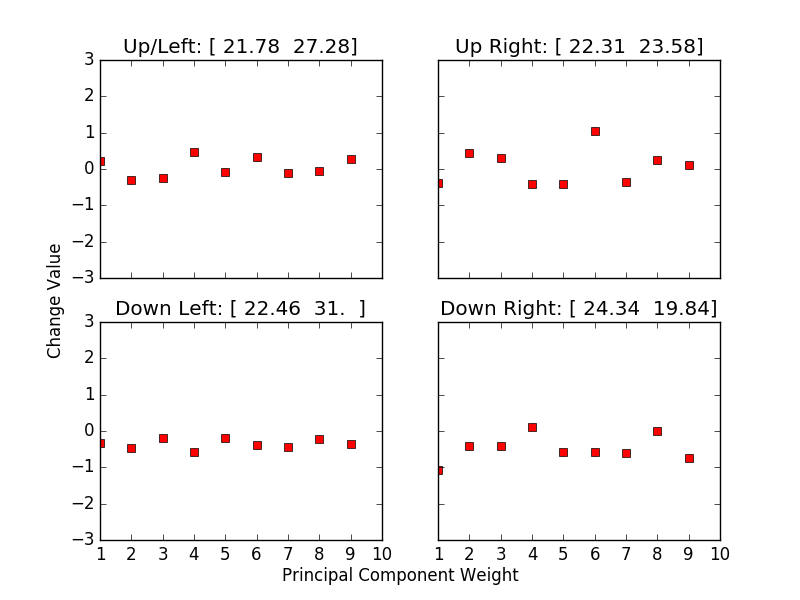
\includegraphics[scale=0.75]{pcw_change_directions}
	}
\end{figure}

There is a slight disconnect in the results as they appear on the chart representing up-right perceptual changes, compared to the others. The average apparent change in that direction is similar to the other three, but the changes made to the PCWs appear much more sweeping. More pair objects were filtered out for this quadrant than any other, from a set that was already the smallest of the four, so it's likely that with more data this graph would be as smooth as the others. 

From this small initial chunk of analysis we can see that there does appear to be a distinct combination of PCW adjustments that results in the kind of positional change denoted by their categorisation. However, because the different adjustments use different combinations of the same weights, there will no doubt be overlap when trying to apply this in practice. Adjusting the PCWs for an HRTF according to the values in the up-left chart might not simply move the source up and left, because some of the changes are shared by multiple directions. For example in this case, the adjustments to the first five PCWs to attempt to move the source position up and left are very similar to the adjustments made to the first five PCWs in a down-right movement. The first PCW, which contains the most information and is most influential in the eventual reconstruction, is adjusted in the opposite direction in each one, so the combinations are distinct overall, but it is not yet known how much of an effect this may have in any resulting perceptual tests. Similarly, in the down-left and up-right adjustments, we see similar values for the first and fourth PCWs, and differences in PCWs two, three, and five. These similarities are the inverse of those on the up-left and down-right charts, which is promising, suggesting a neat correlation might exist when positioning sources towards these quadrants. I have omitted discussion of PCWs six to ten so far, primarily because of their comparatively minimal influence, but it is worth noting that in both the up-left and up-right directions the value of PCW six is increased, though comparatively minimally in the up-left case, possibly indicating some effect on perception. There is a similar link in both the down-left and down-right directions, in which the eighth PCW is increased slightly. Though this adjustment is a lot less pronounced, so further research should be done to confirm any correlation.